\documentclass[11pt, a4paper]{article}

\usepackage[margin=1in]{geometry}
\usepackage{amsmath}
\usepackage{amssymb}
\usepackage{amsthm}
\usepackage{graphicx}
\usepackage{booktabs}
\usepackage{authblk}
\usepackage[numbers]{natbib}
\usepackage[hidelinks]{hyperref}

% Figures live in docs/figures and are regenerated by scripts/05_figures.py.
% Pointing at them rather than copying keeps one source of truth, so
% scripts/11_check_artefacts.py can tell when a figure has gone stale.
\graphicspath{{../docs/figures/}}

\newtheorem{proposition}{Proposition}
\newtheorem{corollary}{Corollary}

\newcommand{\Abar}{\bar{A}}
\newcommand{\Bbar}{\bar{B}}

\title{A Closed-Form Inductive Invariant for\\ Selective State Space Models}

\author[1]{Jack Humphries}
\author[2]{Daniel Midgley}

\affil[1]{Department of Computer Science, University of Surrey}
\affil[2]{Department of Mathematics, University of Surrey}

\date{}

\begin{document}
\maketitle

\begin{abstract}
\noindent Certifying a recurrent model usually means fixing a sequence length,
unrolling the recurrence into a feed-forward network, and calling a verifier. The
resulting certificate holds at that one length only, and it loosens as the length
grows. We show that a selective state space model, the recurrence at the core of
Mamba, needs no unrolling. Under the exact zero-order hold, each state update is a
convex combination of the previous state and an input-dependent equilibrium, so a
bound on the equilibrium is a forward-invariant box for the hidden state. The box is
closed form in the model's own parameters, it holds at every sequence length, and it
requires nothing of the timescale beyond positivity. Its one premise, that the
equilibrium stays bounded, is discharged by the model's own layer normalisation, so
the box holds for every input. The argument is formalised in Isabelle/HOL: the
discretisation identity, the induction, and the normalisation bounds, proved at every
width rather than checked at ours. On a two-layer model trained on limit order book
data, the invariant is 95 times tighter than the fixed point of the standard interval
recursion. The unrolled bound climbs two orders of magnitude towards that fixed point
between ten steps and five thousand; the invariant does not move at all. The ratio
between the invariant and the fixed point has a closed form containing no trained
weight, and it matches the measured value elementwise. Gradient attacks on the trained
model find no violation. The constrained parametrisation costs no measurable accuracy,
so the bound is not bought with performance. The invariant bounds reachable states and
outputs; it is not a robustness guarantee.
\end{abstract}

\section{Introduction}

A selective state space model carries exactly one tensor that accumulates across
timesteps. Every other intermediate inside a block is a fixed-depth function of the
current position and a handful of its neighbours, so a bound on the layer input gives a
bound on it directly. The recurrent state is the exception, and any bound on it has to
survive an arbitrary number of steps.

The standard way to obtain such a bound is to fix a sequence length, unroll the
recurrence into a feed-forward network of that depth, and propagate an input box through
the result. This is sound, and it is what interval and linear-relaxation methods do when
they are pointed at a recurrent model. It also has two costs that are easy to state and
hard to avoid. The certificate is valid at the length it was computed for and at no
other. And it decays with that length: on the model we certify in
Section~\ref{sec:experiments}, the unrolled state bound runs from $127.56$ at $L = 10$ to
$1.226 \times 10^{4}$ at $L = 5000$, while nothing about the network has changed. A model
reading a live stream has no $L$ at all, so there is nothing for this route to certify.

The alternative is an inductive invariant: a set the state begins inside and provably
cannot leave, established once and valid at every length. Invariants for neural sequence
models are not new, and we make no claim on the idea. What we contribute is that for a
selective state space model the invariant need not be searched for at all. It can be
written down in closed form from the discretisation, and its single premise can be
discharged from the architecture rather than assumed of the data.

The mechanism is an identity rather than a technique. Under the exact zero-order hold the
factor $1 - \Abar$ appears in the input gain and as the complement of the transition at
the same time, so the update
\[
  h_t = \Abar_t\, h_{t-1} + (1 - \Abar_t)\, c_t
\]
is a convex combination of the previous state and an input-dependent equilibrium $c_t$. A
convex combination of two quantities lying in $[-M, M]$ lies in $[-M, M]$. A bound on
$c_t$ is therefore already a bound on $h_t$, by induction, at every length, with no
constraint on the timescale beyond positivity. The radius is $M = \sup|Bu|/|A|$, an
expression in the trained parameters and the input box, which can be evaluated once and
quoted.

We claim the following.

\begin{itemize}
  \item A forward-invariant box for the state of a selective state space model, derived
    in closed form from the exact zero-order hold (Section~\ref{sec:invariant}). It holds
    at every sequence length and requires no lower bound on the timescale, and we show
    why the standard separated argument cannot reach it.
  \item A discharge of its premise from the model's own layer normalisation
    (Section~\ref{sec:premise}), so the certificate holds for every input in
    $\mathbb{R}^{L \times d}$ rather than for a data-dependent subset. The fused
    normalisation bound we use for this is tight, not merely sound.
  \item A closed form for the loss the standard interval argument incurs
    (Section~\ref{sec:gap}). It contains no trained weight, which we confirm against the
    trained model elementwise and across random initialisations.
  \item A machine-checked development of the whole chain in Isabelle/HOL
    (Section~\ref{sec:formal}), covering the transcendental steps and the normalisation
    bounds at every width.
  \item Measurements against the alternatives on a trained model
    (Section~\ref{sec:experiments}), and an explicit account of what the certificate does
    not establish (Section~\ref{sec:limitations}).
\end{itemize}

Limit order book forecasting is the demonstration throughout, and only that. The claim is
about the architecture: certification consumes no data, and the predictive numbers appear
solely to establish that the model being certified is a working model rather than an
arbitrary set of weights.

\section{The block, and what varies with time}
\label{sec:block}

A selective state space model computes, at every position, a timescale $\Delta$ together
with matrices $B$ and $C$, all three from the layer input, and then discretises a
diagonal, strictly negative continuous-time $A$ using that timescale
\citep{gu2023mamba}. The block we certify computes
\begin{align*}
  x_n           &= \mathrm{LayerNorm}(x) \\
  [u_0, g]      &= \mathrm{in\_proj}(x_n) \\
  u             &= \mathrm{SiLU}\!\left( \mathrm{DepthwiseCausalConv1d}(u_0) \right) \\
  [p, B, C]     &= \mathrm{x\_proj}(u) \\
  \Delta        &= \Delta_{\min}\left( \Delta_{\max} / \Delta_{\min} \right)^{\sigma(\mathrm{dt\_proj}(p))} \\
  A             &= -\exp(A_{\log}) \\
  \Abar_t       &= \exp(\Delta_t A),
  \qquad
  \Bbar_t        = A^{-1}\!\left( \exp(\Delta_t A) - I \right) B_t \\
  h_t           &= \Abar_t\, h_{t-1} + \Bbar_t\, u_t,
  \qquad h_{-1} = 0 \\
  y_t           &= \textstyle\sum_n C_{t,n}\, h_{t,:,n} + D\, u_t \\
  \mathrm{out}  &= \mathrm{out\_proj}\!\left( y \odot \mathrm{SiLU}(g) \right) + x
\end{align*}
with all products elementwise and broadcast over the state axis. Because $A$ is diagonal,
one memory cell is one scalar recurrence and a block is $d_{\mathrm{inner}} \times
d_{\mathrm{state}}$ independent copies of it. Every statement below is made per cell, and
the block is their product.

The distinction that governs everything else is which of these are weights. Only
$A_{\log}$ and $D$ are. The timescale $\Delta$ and the matrices $B$ and $C$ are
activations, recomputed from the block's own input at every position, so the recurrence is
linear but time-varying and no argument may appeal to time invariance. This is not a
subtlety of presentation. A block's saved parameters contain no $\Delta$, no $B$ and no
$C$ at any position, so a verifier handed the checkpoint and asked to reason about
$\dot h = Ah + Bu$ cannot supply $B$: the tensor does not exist until an input arrives.
What is fixed across inputs is the chain of weights that manufactures those activations,
and a bound must therefore hold uniformly over everything that chain is capable of
emitting.

Two facts hold by construction rather than by training, and both are used below.
$A = -\exp(A_{\log})$ is strictly negative for every real $A_{\log}$, and $\Delta$ is
strictly positive under either parametrisation we consider: the bounded arm written above,
and the reference arm $\Delta = \mathrm{softplus}(z)$, which imposes no lower bound
whatsoever. Neither fact depends on the trained weights, which is what allows the
certificate to be stated for the architecture and not merely for a checkpoint.

\section{A closed-form inductive invariant}
\label{sec:invariant}

\subsection{The discretisation identity}

\begin{proposition}[Discretisation identity]
\label{prop:zoh}
For diagonal $A < 0$ and $\Delta > 0$, the exact zero-order hold gives
\[
  \Abar = \exp(\Delta A),
  \qquad
  \Bbar = A^{-1}\!\left( \exp(\Delta A) - I \right) B = \frac{(1 - \Abar)\, B}{|A|}.
\]
\end{proposition}

\begin{proof}
Read elementwise, and let $a < 0$ be a diagonal entry of $A$. Holding $u$ constant across
a step of length $\Delta$ gives the input multiplier $(\exp(\Delta a) - 1)/a$. Since
$a = -|a|$,
\[
  \frac{\exp(\Delta a) - 1}{a}
    = \frac{1 - \exp(\Delta a)}{|a|}
    = \frac{1 - \Abar}{|a|}. \qedhere
\]
\end{proof}

The proposition is a rearrangement and nothing more, which is precisely why it is
available for every parameter value the block can take. Its content is that the factor
$1 - \Abar$ occupies the input gain and the complement of the transition simultaneously.
That coincidence is what the rest of the paper spends.

It belongs to the exact discretisation rather than to state space models in general. The
forward Euler surrogate $\Bbar \approx \Delta B$ satisfies the identity only in the limit
$\Delta \to 0$. Across the trained timescale range, where $\max|\Delta A| = 1.684$, the
two disagree by $17.3\%$ median and $106.8\%$ maximum relative error, so a model that
discretises approximately is not covered by anything that follows. This is a real
restriction and we state it as one: the invariant is a property of the exact zero-order
hold, and an implementation must earn it.

\subsection{The convex form, and the invariant}

Substituting Proposition~\ref{prop:zoh} into the recurrence gives
\begin{equation}
\label{eq:convex}
  h_t = \Abar_t\, h_{t-1} + (1 - \Abar_t)\, c_t,
  \qquad
  c_t = \frac{B_t\, u_t}{|A|}.
\end{equation}
Since $A < 0$ strictly and $\Delta > 0$, the weight $\Abar_t = \exp(\Delta_t A)$ lies in
$(0,1)$ elementwise, for every parameter value and every input. Each coordinate of $h_t$ is
therefore a convex combination of where the state was and $c_t$, the value it is being
pulled towards. Nothing about this depends on training, and nothing about it depends on
$t$.

\begin{proposition}[Forward invariance]
\label{prop:invariant}
Suppose $|c_t| \le M$ elementwise for every admissible input and every $t$, and that
$h_{-1} = 0$. Then $|h_t| \le M$ for every $t$.
\end{proposition}

\begin{proof}
Write $a$ for a coordinate of $\Abar_t$, so that $a \in (0,1)$. The base case is
$h_{-1} = 0$. Assuming $|h_{t-1}| \le M$,
\[
  |h_t| = \left| a\, h_{t-1} + (1-a)\, c_t \right|
        \le a\,|h_{t-1}| + (1-a)\,|c_t|
        \le a M + (1-a) M = M. \qedhere
\]
\end{proof}

The bound holds at every sequence length because the argument is a single step applied $t$
times and $M$ does not depend on $t$. Nothing is unrolled, and no geometric series is
summed. The only requirement on the timescale is $\Delta > 0$; a lower bound on it buys
nothing here, which is a point we return to with measurements in
Section~\ref{sec:experiments}.

Two strengthenings come for free, and both are formalised in Section~\ref{sec:formal}. The
induction goes through for $a \in [0,1]$ rather than the open interval, which covers the
two degenerate limits a careful reader will reach for: a timescale large enough to flush
the state to $c_t$, and one underflowing to exactly zero, where the state is held. From an
arbitrary initial state the same argument yields $|h_t| \le \max(|h_{-1}|, M)$, so a
deployment carrying state across window boundaries remains certified. Once the state is
inside the box it never leaves, which is the property a streaming system actually needs.

\subsection{Why the separated argument cannot reach this}
\label{sec:separate}

It is worth being precise about what the standard route loses, because the same loss
recurs in Section~\ref{sec:gap} as a measurable quantity and again in
Section~\ref{sec:related} as an obstruction.

Bounding $\Abar$ and $\Bbar$ independently gives
$|h_t| \le s\,|h_{t-1}| + M_{\mathrm{drive}}$ with $s = \sup \Abar$ and
$M_{\mathrm{drive}} = \sup|\Bbar u|$, hence $|h| \le M_{\mathrm{drive}}/(1 - s)$. But
$M_{\mathrm{drive}}$ carries the factor $1 - \Abar$ and is taken at its maximum, so the
numerator holds $1 - \inf\Abar$ while the denominator holds $1 - \sup\Abar$. The
cancellation visible in~\eqref{eq:convex} is destroyed. As $\Delta \to 0$ both factors
vanish at the same rate and the true ratio is stable, while the separated bound diverges;
nothing about the state is diverging, and the divergence is an artefact of having bounded
the two occurrences of $\Abar$ as though they were unrelated.

The same dependency loss prevents the induction step itself from being checked by interval
arithmetic. In $a h + (1-a) c$ the variable $a$ occurs twice. An interval evaluator bounds
the two products independently, permitting the first to take $\sup\Abar$ while the second
takes $1 - \inf\Abar$; the weights then sum past one, the step reports growth, and the
check fails for every box that is not a single point. Keeping $a$ as one variable, the
supremum over $a \in [0,1]$ of $aM + (1-a)M_c$ is $\max(M, M_c)$, so the box is preserved
exactly when $M_c \le M$. We report $\max(M, M_c) - M$ as a residual, and check it rather
than assume it.

\section{Discharging the premise}
\label{sec:premise}

Proposition~\ref{prop:invariant} assumes the equilibrium stays inside a box. Because $B$
and $u$ are activations, that premise has to hold for every input the model could ever
receive, not for the inputs some dataset happens to contain. Assuming it of the data would
make the certificate conditional on a distribution and worth much less. The architecture
supplies it instead, because every block opens with a layer normalisation whose output
lies in a box fixed by its own parameters.

\begin{proposition}[Coordinate bound]
\label{prop:ln}
For a layer normalisation with normalised shape $d$ and $\varepsilon > 0$, every
$x \in \mathbb{R}^{d}$ and every coordinate $i$ satisfy
\[
  \left| \mathrm{LN}(x)_i - \beta_i \right| \le |\gamma_i|\,\sqrt{d-1}.
\]
\end{proposition}

\begin{proof}
Write $z = (x - \mu)/\sqrt{\sigma^2 + \varepsilon}$, so that
$\mathrm{LN}(x) = \gamma \odot z + \beta$. Normalisation forces $\sum_j z_j = 0$ and
$\sum_j z_j^2 = d\,\sigma^2/(\sigma^2 + \varepsilon) \le d$. Fix $i$ and set $c = z_i$.
The zero sum gives $\sum_{j \ne i} z_j = -c$, and Cauchy--Schwarz over the remaining
$d - 1$ coordinates gives $\sum_{j \ne i} z_j^2 \ge c^2/(d-1)$. Adding $c^2$ to both sides
and comparing with the energy constraint yields $d \ge c^2 d/(d-1)$, hence
$c^2 \le d - 1$. Scaling by $\gamma_i$ and shifting by $\beta_i$ gives the claim.
\end{proof}

The proof mentions neither $x$ nor its scale, so the bound holds for inputs no order book
would ever produce. Informally, pushing one coordinate high requires the other $d-1$ to
cancel it, and that cancellation is paid for out of a fixed energy budget. Note also that
the $\varepsilon$ in the denominator works in our favour: it makes the energy constraint an
inequality rather than an equality, so the bound is conservative in the correct direction.

Stating the bound coordinatewise, however, throws away the two constraints that produced
it. Retaining them costs nothing and yields a bound that cannot be improved.

\begin{proposition}[Fused bound, and its attainment]
\label{prop:fused}
Let $v_k = W_k \odot \gamma$ and let
$S = \{\, z : \mathbf{1}^{\top} z = 0,\ \|z\|_2 \le \sqrt{d} \,\}$. Then
\[
  \sup_{z \in S} \langle v_k, z \rangle
    = \left\| v_k - \bar{v}_k \mathbf{1} \right\|_2 \sqrt{d},
\]
attained at
$z^{\ast} = \sqrt{d}\,(v_k - \bar{v}_k \mathbf{1}) / \|v_k - \bar{v}_k \mathbf{1}\|_2$.
\end{proposition}

\begin{proof}
Since $\mathbf{1}^{\top} z = 0$, the constant vector $\bar{v}_k \mathbf{1}$ is orthogonal
to $z$, so the mean subtracts for free and
$\langle v_k, z \rangle = \langle v_k - \bar{v}_k \mathbf{1},\, z \rangle$.
Cauchy--Schwarz over $\|z\|_2 \le \sqrt{d}$ gives the bound. The candidate $z^{\ast}$ sums
to zero and has norm exactly $\sqrt{d}$, so it lies in $S$, and substituting it returns the
bound with equality.
\end{proof}

Fusing the normalisation with the linear map that follows it therefore gives a bound that
is tight over $S$ rather than merely sound. Bounding the two layers separately gives
$\|v_k\|_1\sqrt{d-1}$, which is an $\ell_1$ quantity where an $\ell_2$ one suffices and
discards the zero-sum constraint besides. The difference is not cosmetic, because the
radius is $\sup|Bu|/|A|$ and the cost lands on it directly. On the trained model the fused
bound gives $\sup|u| = 8.4267$ and a radius of $129.6739$, against $61.3134$ and
$6332.03$ for the coordinatewise route: a factor of $48.8$. Keeping the convolution
depthwise rather than channel-mixing is worth a further factor of $71$. Neither choice
affects whether the invariant exists, only how much it is worth.

What remains is mechanical. An interval domain carries the normalisation box through the
projections, the depthwise causal convolution and the activations to boxes on $B$ and $u$,
and hence to $M$. Every abstract transformer obeys one contract: given boxes containing
its inputs, it returns a box containing every output those inputs can produce. Three
operations need more than endpoint evaluation. The SiLU activation has an interior minimum,
so a box straddling it cannot be bounded from its endpoints alone. The causal convolution
must hull its input box with zero, because the block left-pads with zeros and zero need not
lie in the box on $u$; omitting this fails only at the first few positions, which sampling
from the middle of a sequence would never reveal. And the product of two intervals is taken
over its four corners, which is exact for independent factors. $B$ and $u$ are not
independent, and that discard is where most of the remaining looseness lives
(Section~\ref{sec:experiments}).

\section{The abstraction gap in closed form}
\label{sec:gap}

The loss identified in Section~\ref{sec:separate} can be written down exactly rather than
merely observed. Writing $\lambda = |A|$ and the propagated timescale box as
$[\delta_{\mathrm{lo}}, \delta_{\mathrm{hi}}]$,
\[
  \text{invariant} = \frac{\sup|Bu|}{\lambda},
  \qquad
  \text{geometric}
    = \frac{\left(1 - e^{-\lambda \delta_{\mathrm{hi}}}\right)\sup|Bu| \,/\, \lambda}
           {1 - e^{-\lambda \delta_{\mathrm{lo}}}},
\]
because $\sup|\Bbar u|$ carries the factor $1 - \inf\Abar$ while the denominator carries
$1 - \sup\Abar$. Every term except $\lambda$ cancels between them:
\begin{equation}
\label{eq:gap}
  \mathrm{gap}(\lambda)
    = \frac{1 - e^{-\lambda \delta_{\mathrm{hi}}}}{1 - e^{-\lambda \delta_{\mathrm{lo}}}}.
\end{equation}

Three consequences follow, and each is visible in the sweep reported in
Section~\ref{sec:experiments}. The expression contains no trained weight, so the ratio is
stable to three figures across random initialisations while the radius itself moves by
roughly thirty percent. It increases as $\lambda$ falls, so the slowest pole attains it.
And it grows like $1/\delta_{\mathrm{lo}}$, which is why lowering the timescale floor by a
decade costs the separated bound a factor of ten and costs the invariant nothing at all.
Equation~\eqref{eq:gap} is bounded below by $1$ for any nondegenerate timescale box, so
the separated bound never beats the invariant, at any pole and any timescale range.

We regard this as the part of the work that behaves like a prediction rather than a
measurement. Equation~\eqref{eq:gap} was derived before it was compared against the
certificate, it could have disagreed, and Section~\ref{sec:experiments} reports what
happened instead.

\section{Machine-checked proof}
\label{sec:formal}

% ---------------------------------------------------------------------------
% DANIEL: this section is yours to write. Notes, not text:
%
%   - the theory is isabelle/Mamba_Invariant.thy, session MambaVLob, Isabelle2025-2
%   - 442 commands, no errors, no sorries; imports only Complex_Main (no AFP)
%   - the five statements map to: convex_combination_bound; Abar_in_unit_interval
%     (+ _closed); zoh_identity and update_is_convex_combination;
%     convex_recurrence_invariant with headline mamba_cell_state_bounded;
%     layernorm_bound, fused_layernorm_linear_bound, fused_layernorm_linear_attained
%   - beyond the five: zoh_is_exact_flow, abstraction_gap_ge_one,
%     A_parametrisation_negative, softplus_positive, bounded_dt_positive
%   - Cauchy-Schwarz for finite sums is not in Complex_Main, so the theory proves it
%   - worth stating plainly what a machine-checked proof does and does not buy:
%     Isabelle guarantees the proofs, not that the statements are the intended ones
%   - the theory's own Scope section is the honest list of what is out of scope
% ---------------------------------------------------------------------------

\textit{[To be written by D.M.]}

\section{Relation to invariant inference and reachability}
\label{sec:related}

% ---------------------------------------------------------------------------
% DANIEL: this section is yours. Facts below were checked against the primary
% source (Jacoby, Barrett & Katz, ATVA 2020; full version arXiv:2004.02462) on
% 1 September 2026, so they can be relied on:
%
%   - their step is  v_i^t = f(W_i v_{i-1}^t + H_i \tilde{v}_i^t + b_i)  with f = ReLU,
%     i.e. the recurrence enters through H on the memory unit, and there is a bias.
%     (NOT ReLU(Wv + Ux) as an earlier draft of ours had it.)
%   - they state the class limit themselves, verbatim: "While we focus here on vanilla
%     RNNs, our technique could be extended to, e.g., LSTMs or GRUs; we leave this for
%     future work." Quoting them is stronger than asserting it ourselves.
%   - backend is Marabou: "uses the Marabou tool as its FFNN verification back-end"
%   - the loop "terminates when the property is proven correct, when a counter-example
%     is found, or when a certain timeout value is exceeded", and in the last case the
%     results are explicitly "inconclusive"
%   - the invariant template is affine in time:  alpha_l (t-1) <= v~^t <= alpha_u (t-1)
%
% The contrast worth drawing, which our earlier framing missed: their invariants are
% permitted to GROW with t by construction, ours is constant in t. That is a difference
% in the shape of the certificate, not only in its tightness.
%
% Also for this section: Tran et al. (star sets) as the strongest representative of the
% unrolling route; and Bonassi et al., where the correct contrast is NOT
% "training vs construction" (a GRU's box is structural too, since the activation caps
% it) but that a GRU's box is the activation's range, a constant, whereas ours is a
% closed form in the trained weights that moves with the model.
% ---------------------------------------------------------------------------

\textit{[To be written by D.M.]}

\section{Experiments}
\label{sec:experiments}

\subsection{Setup}

We train a two-layer selective state space model with $d_{\mathrm{model}} = 64$,
$d_{\mathrm{state}} = 16$, $d_{\mathrm{inner}} = 128$, $d_{\mathrm{conv}} = 4$,
$\mathrm{dt\_rank} = 4$ and $\Delta \in [10^{-3}, 10^{-1}]$, on limit order book data:
Databento MBP-10 from Nasdaq TotalView-ITCH, one instrument on one day, $4{,}550{,}476$
rows after feature construction and $43$ model inputs. The three-way chronological split
is purged by $100$ ticks at each boundary, so no window straddles a split. Features are
winsorised to train-split quantiles at inference rather than only during training, which
makes the standardised input box $[-6.60, 18.87]$ a deployment guarantee rather than a
historical observation; there are no violations across all rows. On the trained weights
$A$ spans $[-16.8437, -0.9651]$.

None of the certification depends on any of this. The invariant is a statement about the
architecture and the trained weights, it consumes no data, and it holds for inputs no
order book would produce.

\subsection{The invariant against the alternatives}

Table~\ref{tab:alternatives} reports the certified state bound at $L = 100$. The widened
column iterates generic interval propagation to convergence, taking $10{,}509$ iterations
at layer~0 and $10{,}634$ at layer~1, and lands on the geometric fixed point as it should;
we report it rather than a truncated unrolling so that the comparison is against the best
the standard route can do rather than against an arbitrary stopping point. Induction holds
in both layers with residual exactly zero, and the discretisation identity checks exact.

\begin{table}[ht]
\centering
\begin{tabular}{@{}lrrrr@{}}
\toprule
Layer & Invariant & Widened fixed point & Unrolled, $L = 100$ & Tighter by \\
\midrule
0 & $129.6739$ & $1.235 \times 10^{4}$ & $1169.03$ & $95.23\times$ \\
1 & $143.5443$ & $1.368 \times 10^{4}$ & $1273.92$ & $95.31\times$ \\
\bottomrule
\end{tabular}
\caption{Certified $\sup|h|$ from the invariant and from the alternatives, computed
  without data.}
\label{tab:alternatives}
\end{table}

\subsection{Scaling with sequence length}

\begin{figure}[htbp]
  \centering
  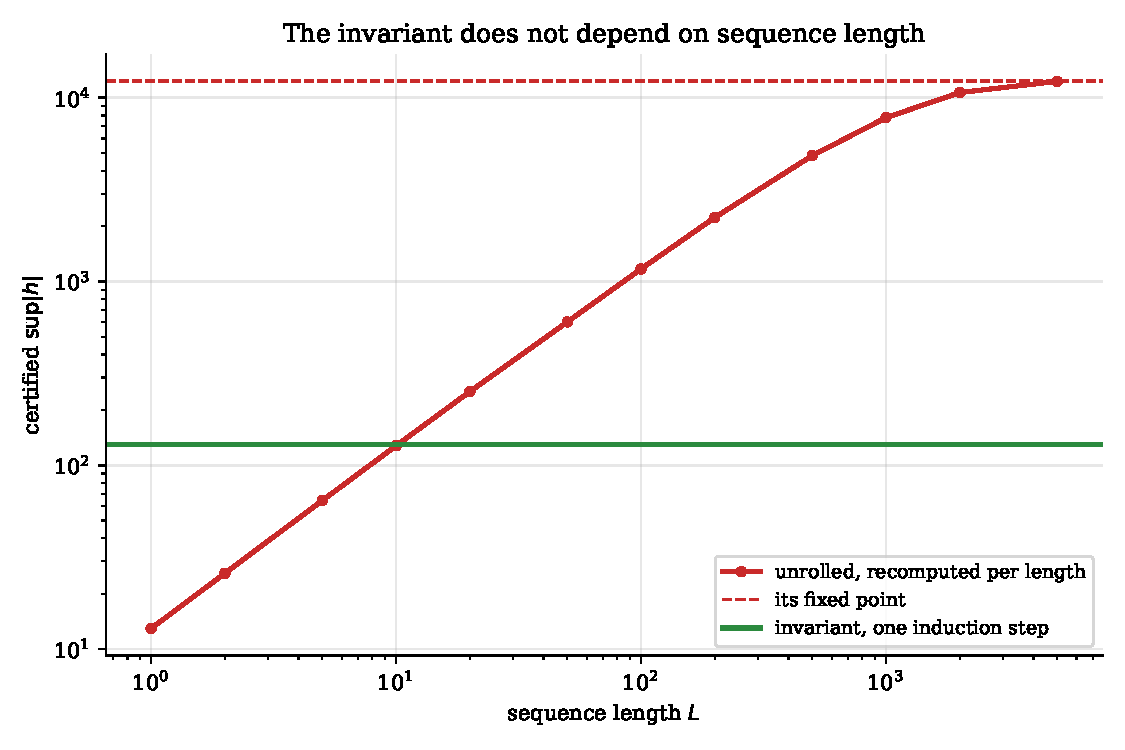
\includegraphics[width=0.75\textwidth]{bound_vs_horizon.pdf}
  \caption{Certified bound on the state against sequence length, layer~0. The unrolled
    interval bound is recomputed at each length and climbs towards its fixed point; the
    invariant is one induction step and does not move. The two cross at about $L = 10$.}
  \label{fig:horizon}
\end{figure}

The invariant is $129.67$ at $L = 10$ and $129.67$ at $L = 5000$. Across the same range
the unrolled bound runs $127.56$, $601.78$, $1169.03$, $4838.40$, $7781.12$ and
$1.226 \times 10^{4}$ at $L = 10, 50, 100, 500, 1000, 5000$ respectively, which is
Figure~\ref{fig:horizon}. Below
$L \approx 10$ the unrolled bound is the tighter of the two, which we state because it is
true and because it locates precisely where the tradeoff turns: the invariant is not
uniformly better, it is better everywhere past a handful of steps and it stops moving.

\subsection{No floor on the timescale}

With $\Delta = \mathrm{softplus}(z)$, which admits no lower bound at all, induction still
holds and the invariant certifies at $129.7168$ and $143.3978$. The separated argument on
the same model gives $1.298 \times 10^{7}$ and $1.433 \times 10^{7}$, because
$\sup\Abar = 1$ and it is dividing by $1 - \sup\Abar$. The invariant needs no floor on the
timescale; only the geometric argument ever did. Figure~\ref{fig:floor} sweeps the floor
directly.

\begin{figure}[htbp]
  \centering
  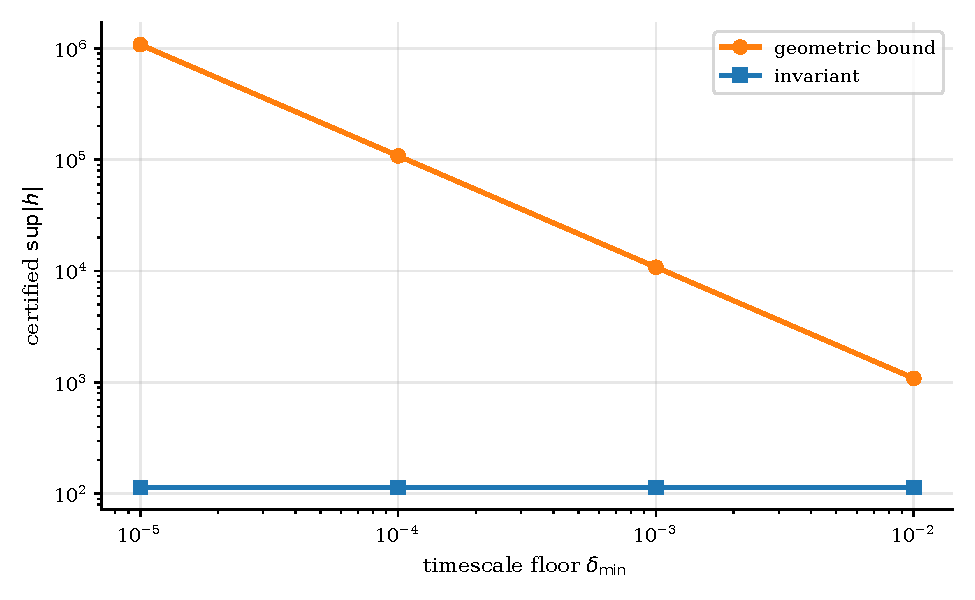
\includegraphics[width=0.75\textwidth]{bound_vs_floor.pdf}
  \caption{Certified $\sup|h|$ as the timescale floor $\Delta_{\min}$ is lowered,
    layer~0, at a fixed random initialisation; moving the floor changes the
    architecture, and the trained checkpoint exists at one floor only. The geometric
    bound pays a factor of ten per decade of floor; the invariant does not move.}
  \label{fig:floor}
\end{figure}

\subsection{The gap formula against measurement}

\begin{figure}[htbp]
  \centering
  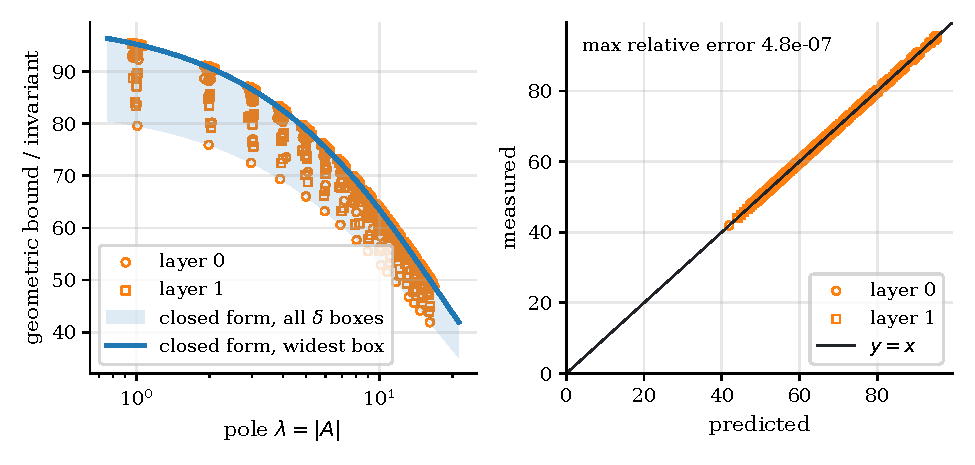
\includegraphics[width=\textwidth]{gap_prediction.pdf}
  \caption{The abstraction gap for every (channel, state) element of the trained model.
    Left: against the pole $\lambda$, with equation~\eqref{eq:gap} drawn over the
    propagated timescale boxes. Right: predicted against measured. Maximum relative error
    $4.8 \times 10^{-7}$.}
  \label{fig:gap}
\end{figure}

Equation~\eqref{eq:gap} reproduces the measured ratio elementwise to $5 \times 10^{-7}$,
plotted per element in Figure~\ref{fig:gap}. Across eight random initialisations the ratio moves between $95.203$ and $95.209$ while
the radius itself moves between $101.2$ and $132.2$, which is the weight-independence
of~\eqref{eq:gap} made visible: the quantity the formula predicts is stable precisely
where the quantity it does not predict is not. Figure~\ref{fig:seeds} plots both on one
scale. Induction holds in all $29$ configurations swept.

\begin{figure}[htbp]
  \centering
  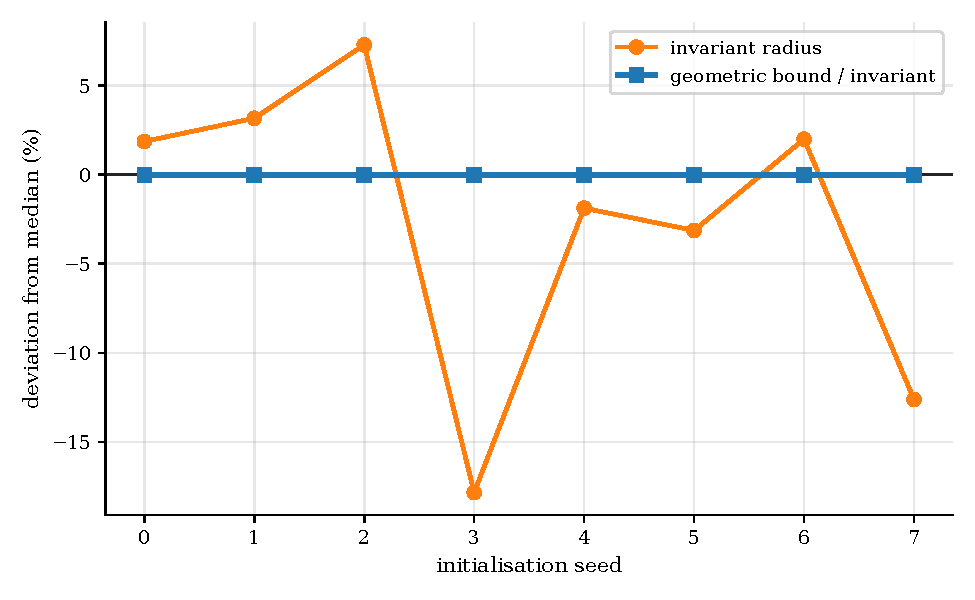
\includegraphics[width=0.75\textwidth]{sweep_seeds.pdf}
  \caption{Eight random initialisations, each series shown as the deviation from its own
    median. The invariant radius moves with the weights by roughly thirty percent; the
    ratio of the geometric bound to the invariant, the quantity fixed by
    equation~\eqref{eq:gap}, moves by less than a hundredth of a percent.}
  \label{fig:seeds}
\end{figure}

\subsection{Tightness and falsification}

Gradient ascent on the input, run against each certified quantity in the unrestricted
regime where the normalisation bound is the only thing holding the certificate up, finds
no violation. Optimising against a bound also prices it, since
$\text{attacked} \le \text{true reachable} \le \text{certified}$, so the same procedure
reports how much room is left. The timescale bounds are near-exact at $1.06\times$ and
$1.09\times$, $\sup|u|$ is $1.78\times$, and the state bound sits $217\times$ above the
attacked value.

That last figure deserves an explanation rather than a defence. Against the certified
boxes the radius is roughly $630$ times the realised state, and the induction is not where
that sits. Recomputing $M$ from a realised trace rather than from the certified boxes gives
$1.0020$ against a realised $\sup|h|$ of $0.2066$ at layer~0, and $0.5139$ against
$0.1585$ at layer~1. The induction therefore accounts for a factor of three to five, and
the boxes on $B$ and $u$ account for the remainder. The dominant term is the interval
product discarding the correlation between $B$ and $u$, which is a known weakness of the
box domain and not a weakness of the invariant. The exported certificate records a wider
realised envelope than the single trace used here, and against it the same radii come out
at $499\times$ and $854\times$; Figure~\ref{fig:priced} reports that ratio for every
certified quantity.

\begin{figure}[htbp]
  \centering
  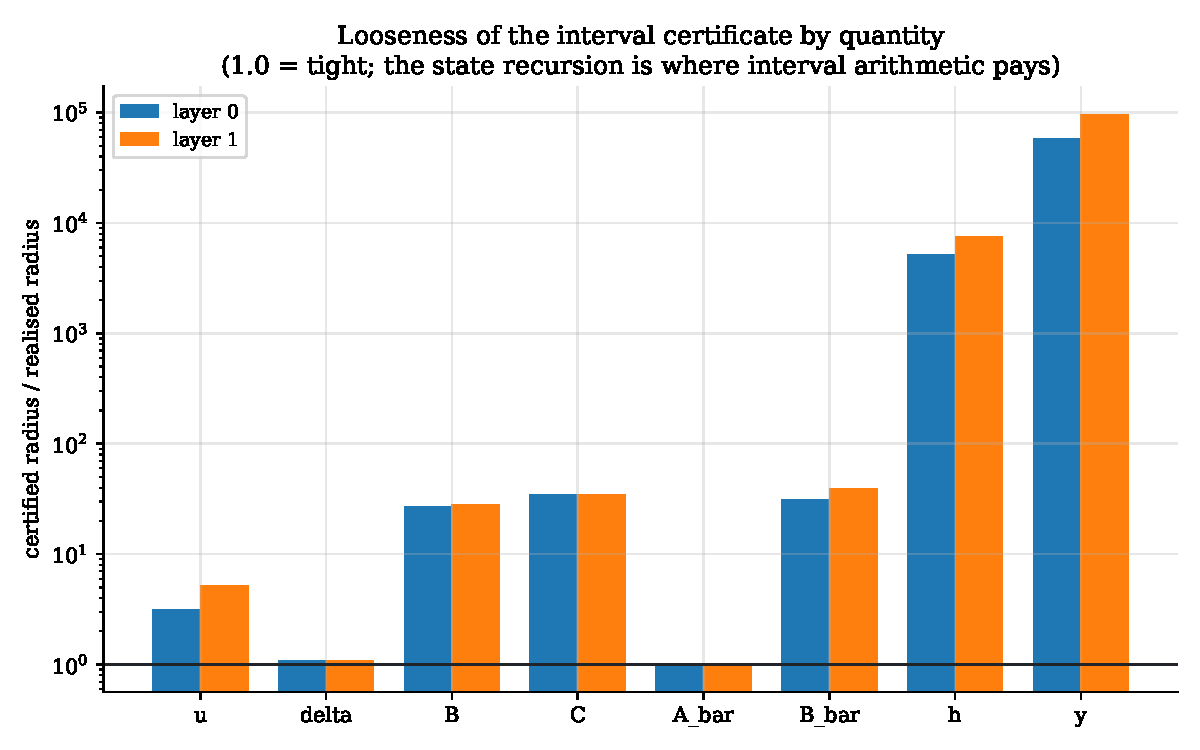
\includegraphics[width=0.7\textwidth]{certified_vs_realised.pdf}
  \caption{Certified radius over realised radius for each certified quantity, both
    layers, log scale. The timescale sits at $1.09\times$ and the transition $\Abar$ at
    $1.0001\times$ and $1.0002\times$; the state carries $499\times$ and $854\times$,
    and the readout $y$ carries $2482\times$ and $4049\times$. The state factor is
    attributable to the boxes on $B$ and $u$ rather than to the induction.}
  \label{fig:priced}
\end{figure}

The whole-network output bound, taken through the final normalisation and therefore
holding for any input in $\mathbb{R}^{L \times 43}$ with no premise at all, is
$[-5.1242, 4.3374]$. One standardised unit is $0.7042$ basis points of the forward return,
so the model cannot emit a forecast outside roughly $[-3.600, +3.063]$ basis points. This
licenses a position limit computed from the weights before the model sees a single tick.
It says nothing whatever about whether the forecast is any good.
Figure~\ref{fig:output} drives the model with white noise up to $10^{6}$ standard
deviations; the output stays inside the certified band.

\begin{figure}[htbp]
  \centering
  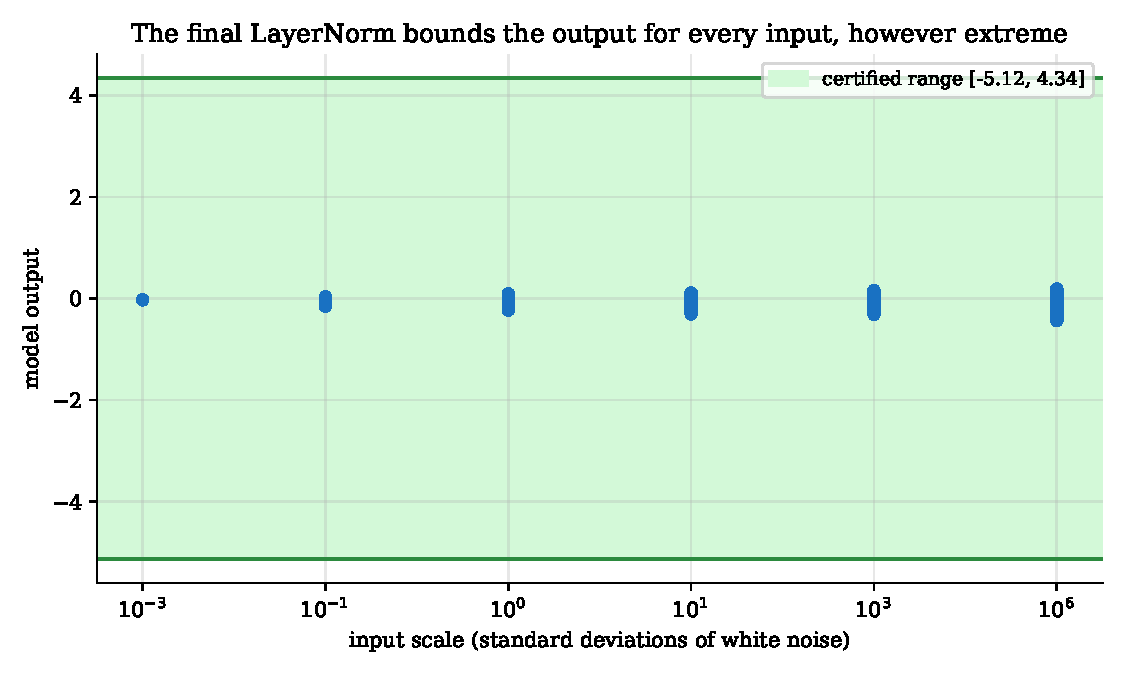
\includegraphics[width=0.7\textwidth]{certified_output_range.pdf}
  \caption{Realised output ranges under white-noise inputs scaled from $10^{-3}$ to
    $10^{6}$ standard deviations, against the certified range $[-5.12, 4.34]$, which
    carries no premise on the input.}
  \label{fig:output}
\end{figure}

\subsection{The certified model is a working model}

Rank information coefficient on the held-out split, over $25{,}600$ overlapping
observations corresponding to $256$ independent windows: LSTM $+0.1111$, the certified
model $+0.1044$, its softplus arm $+0.1043$, a causal transformer $+0.1040$, and ridge
regression $+0.0312$. Standard errors from a circular block bootstrap
\citep{politis1994stationary} are four to five times the naive independent estimate, and
Diebold--Mariano tests \citep{diebold1995comparing} with the Harvey--Leybourne--Newbold
correction \citep{harvey1997testing} separate every neural model from ridge, and separate
the two Mamba arms from each other with the bounded arm favoured; no other pair
separates. Figure~\ref{fig:dm} gives the full grid of pairwise $p$-values.

\begin{figure}[htbp]
  \centering
  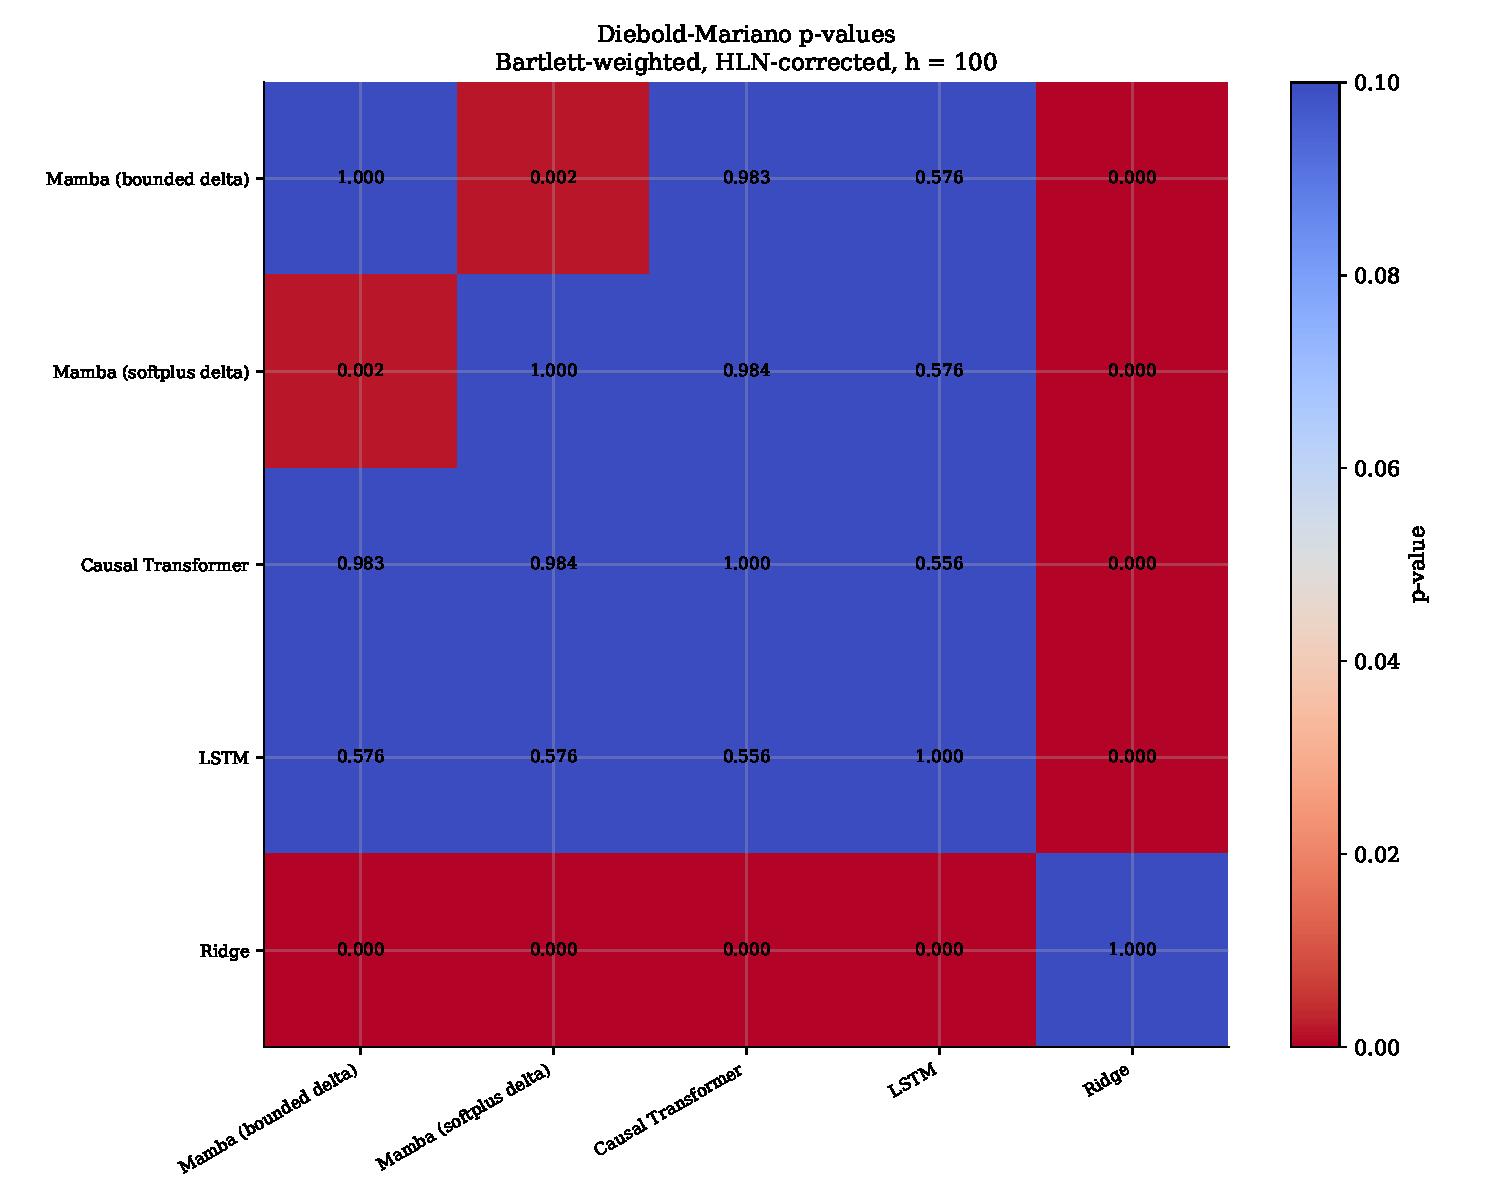
\includegraphics[width=0.8\textwidth]{dm_test_heatmap.pdf}
  \caption{Pairwise Diebold--Mariano $p$-values under the Harvey--Leybourne--Newbold
    correction, computed on overlapping forecasts. Every neural model separates from the
    ridge baseline, and the two Mamba arms separate from each other with the bounded arm
    favoured; no other pair separates.}
  \label{fig:dm}
\end{figure}

The only claim these numbers support is that the constrained parametrisation costs no
measurable accuracy relative to the unconstrained one (the one significant pairwise
difference favours it), so the certificate is not bought with performance. One instrument
on one day supports nothing beyond that, and we draw nothing beyond it.

\subsection{Reproducibility}

The exported certificate is a single file containing the equations, the weights, the
certified boxes and the realised envelope. A NumPy reference implementation reads only
that file, imports nothing from the model, and reproduces the entire forward pass to
$8.8 \times 10^{-7}$ against the PyTorch model, so the artefact can be checked without
trusting our implementation. This check has already earned itself once: an earlier version
of the reference reversed the depthwise convolution kernel, because the underlying
operator cross-correlates rather than convolves, and every bound and every unit test still
passed. Sixteen of nineteen supporting interval lemmas discharge under Z3
\citep{demoura2008z3} with no counterexamples; the remainder are subsumed by the Isabelle
development of Section~\ref{sec:formal}.

\section{Limitations}
\label{sec:limitations}

The certificate bounds reachable states and reachable outputs. It is not a robustness
certificate. Nothing here bounds $|f(x) - f(x')|$ for nearby inputs, and any reading of
these numbers as adversarial robustness is a misreading. A bounded output is likewise not
a bounded loss: the model cannot emit an arbitrarily large forecast, and that is all.

The formal development is over the reals while the model runs in float32. The convex
skeleton survives rounding in a specific sense: a correctly rounded exponential of a
nonpositive argument still lies in $[0,1]$, so the computed weight remains a convex weight
and the induction still applies, with per-step arithmetic error entering additively and
decaying at $\Abar$. The geometric factor the invariant removes from the bound reappears
in the error term, at most $1/(1 - \sup\Abar)$. For the bounded timescale arm this is
negligible against float32 noise. For the softplus arm, where $\sup\Abar = 1$, worst-case
drift grows with $t$, so strict length-independence in floating point is a statement about
the reals unless a floor is reintroduced. We regard this as a finding rather than a flaw,
since it locates exactly where a timescale floor matters and where it does not, but a
restated theorem carrying an explicit error term remains open work.

One further piece of small print belongs here. Our implementation computes
$\phi(v) = \mathrm{expm1}(v)/v$ with a cubic Taylor branch below $|v| = 10^{-4}$, where
the expression is otherwise $0/0$. On that branch the implemented update departs from the
exact zero-order hold by a relative error of order $|v|^3/24 \le 4 \times 10^{-14}$, far
below float32 resolution but nonzero, so the code implements the exact discretisation only
up to that.

Composition across blocks and through the head is performed by interval arithmetic in code
rather than by proof. End to end the output bound is several times looser than what the
model attains, and most of that slack is in the composition rather than in the invariant.
Formalising the interval domain and proving the chain sound by induction over the layers is
the natural continuation of Section~\ref{sec:formal}.

We attempted two local sensitivity domains, and report their failure because it is
informative. Both diverge on inputs where the model is measurably well behaved, one
reaching $10^{24}$ and the other exceeding the unconditional bound above
$\varepsilon = 10^{-5}$. The attacked width is linear in $\varepsilon$ across five
decades, placing the model's true local Lipschitz constant at about $1.63$. The domains
fail, not the model. A relaxation carrying linear coefficients, such as a zonotope, is the
standard remedy and we have not implemented one.

Finally, the predictive comparison is one instrument on one day, no learning-rate sweep
was run, and every model plateaus at its first evaluation. Three architectures at one
setting each is not a comparison of architectures, and we do not offer it as one. The
novelty position in Section~\ref{sec:related} rests on a literature search that was not
exhaustive.

\section{Conclusion}

The hidden state of a selective state space model stays inside a box that can be written
down in closed form from the model's own parameters. The mechanism is the exact zero-order
hold, which makes every update a convex combination of the previous state and a bounded
equilibrium; the premise is discharged by the layer normalisation the architecture already
contains; and the resulting chain is machine-checked. The certificate holds at every
sequence length, requires no lower bound on the timescale, and is roughly ninety-five
times tighter than what generic interval propagation converges to, by a factor we can
write down in advance and confirm elementwise.

What this does not do is also clear, and we have tried to say so plainly throughout. It
bounds reachability rather than robustness, it is stated over the reals rather than over
floating point, and it composes across blocks by code rather than by proof. Each of those
is a well-posed next step rather than an obstacle, and the last two are the ones we would
take first.

\bibliographystyle{plainnat}
\bibliography{references}

\end{document}
